\documentclass[a4paper]{article}

%Пакеты для математических символов:
\usepackage{amsmath} % американское математическое сообщество.
\usepackage{amssymb} % миллион разных значков и готический, ажурный шрифты.
\usepackage{amscd} % диаграммы, графики.
\usepackage{amsthm} % окружения теорем, определений и тд.
\usepackage{physics} % основные физические символы
%\usepackage{latexsym} % треугольники и пьяная стрелка.

%пакеты для шрифтов:
%\usepackage{euscript} % прописной шрифт с завитушками.
\usepackage{MnSymbol} % Значеки доказательства
\usepackage{verbatim} % улучшенный шрифт "пишущей машинки".
%\usepackage{array} % более удобные таблицы.
%\usepackage{multirow} % мультистолбцы в таблицах.
%\usepackage{longtable} % таблицы на несколько страниц.
%\usepackage{latexsym}

\usepackage{etoolbox}
\usepackage{slashbox} %Разделениени текста \backslashbox{}{}
\usepackage{collectbox} % Добавляет коробочки, можно складывать туда текст)

%Пакеты для оформления:
\RequirePackage[center, medium]{titlesec}% Стиль секций и заголовков
%\usepackage[x11names]{xcolor} % 317 новых цветов для текста.
%\usepackage{multicol} % набор текста в несколько колонн.
\usepackage{graphicx} % расширенные возможности вставки стандартных картинок.
\usepackage{subcaption} % возможность вставлять картинки в строчку
%\usepackage{caption} % возможность подавить нумерацию у caption.
\usepackage{wrapfig} % вставка картинок и таблиц, обтекаемых текстом.
\usepackage{cancel} % значки для сокращения дробей, упрощения, стремления.
\usepackage{misccorr} % в заголовках появляется точка, но при ссылке на них ее нет.
%\usepackage{indentfirst} % отступ у первой строки раздела
%\usepackage{showkeys} % показывает label формул над их номером.
%\usepackage{fancyhdr} % удобное создание верхних и нижних колонтитулов.
%\usepackage{titlesec} % еще одно создание верхних и нижних колонтитулов

%Пакеты шрифтов, кодировок. НЕ МЕНЯТЬ РАСПОЛОЖЕНИЕ.
\usepackage[utf8]{inputenc} % кодировка символов.
%\usepackage{mathtext} % позволяет использовать русские буквы в формулах. НЕСОВМЕСТИМО С tempora.
\usepackage[T1, T2A]{fontenc} % кодировка шрифта.
\usepackage[english, russian]{babel} % доступные языки.


%tikz:
\usepackage{tikz} % tikz
\usetikzlibrary{decorations.text} % позволяет делать текст вдоль кривой.
\usetikzlibrary{external} % позволяет кэшировать рисунки tikz.

%Отступы и поля:
%размеры страницы А4 11.7x8.3in
\textwidth=7.3in % ширина текста
\textheight=10in % высота текста
\oddsidemargin=-0.5in % левый отступ(базовый 1дюйм + значение)
\topmargin=-0.5in % отступ сверху до колонтитула(базовый 1дюйм + значение)


%Сокращения
%Скобочки
\newcommand{\inrad}[1]{\left( #1 \right)}
\newcommand{\inner}[1]{\left( #1 \right)}
\newcommand{\infig}[1]{\left{ #1 \right}}
\newcommand{\insqr}[1]{\left[ #1 \right]}
\newcommand{\ave}[1]{\left\langle #1 \right\rangle}


%% Красивые <= и >=
\renewcommand{\geq}{\geqslant}
\renewcommand{\leq}{\leqslant}

%%Значек выполнятся
\newcommand{\per}{\hookrightarrow}



%% Более привычные греческие буквы
\renewcommand{\phi}{\varphi}
\renewcommand{\epsilon}{\varepsilon}
\newcommand{\eps}{\varepsilon}
\newcommand{\com}{\mathbb{C}}
\newcommand{\re}{\mathbb{R}}
\newcommand{\nat}{\mathbb{N}}
\newcommand{\stp}{$\filledmedtriangleleft$}
\newcommand{\enp}{$\filledmedsquare$}

\makeatletter
\newcommand{\sqbox}{%
    \collectbox{%
        \@tempdima=\dimexpr\width-\totalheight\relax
        \ifdim\@tempdima<\z@
            \fbox{\hbox{\hspace{-.5\@tempdima}\BOXCONTENT\hspace{-.5\@tempdima}}}%
        \else
            \ht\collectedbox=\dimexpr\ht\collectedbox+.5\@tempdima\relax
            \dp\collectedbox=\dimexpr\dp\collectedbox+.5\@tempdima\relax
            \fbox{\BOXCONTENT}%
        \fi
    }%
}
\makeatother
\newcommand{\mergelines}[2]{
\begin{tabular}{llp{.5\textwidth}}
#1 \\ #2
\end{tabular}
}
\newcommand\tab[1][0.51cm]{\hspace*{#1}}
\newcommand\difh[2]{\frac{\partial #1}{\partial #2}}
\newcommand{\messageforpeople}[1]{HSE Faculty of Physics \ \ HSE Faculty of Physics HSE Faculty of Physics \ \ HSE Faculty of Physics HSE Faculty of Physics \ \ HSE Faculty of Physics HSE Faculty of Physics \ \ HSE Faculty of Physics HSE Faculty of Physics \ \ HSE Faculty of Physics HSE Faculty of Physics \ \ HSE Faculty of Physics HSE Faculty of Physics \ \ HSE Faculty of Physics HSE Faculty of Physics \ \ HSE Faculty of Physics }


\numberwithin{equation}{section}

\begin{document}

\pagestyle{empty}
\oddsidemargin=-1.18in
\topmargin=-1.5in

\begin{titlepage}
\begin{tikzpicture}
    \draw [white] (0, 0) ellipse (4.1in and 5.7in);
    \path [postaction={
    decoration={text along path,
    text={\messageforpeople{}},
    text align=center,
    raise=0mm,
    reverse path}, decorate}]
    [postaction={
    decoration={text along path,
    text={\messageforpeople{}},
    text align=center,
    raise=3mm,
    reverse path}, decorate}]
    [postaction={
    decoration={text along path,
    text={\messageforpeople{}},
    text align=center,
    raise=6mm,
    reverse path}, decorate}]
    [postaction={
    decoration={text along path,
    text={\messageforpeople{}},
    text align=center,
    raise=9mm,
    reverse path}, decorate}]
    [postaction={
    decoration={text along path,
    text={\messageforpeople{}},
    text align=center,
    raise=12mm,
    reverse path}, decorate}] 
    [postaction={
    decoration={text along path,
    text={\messageforpeople{}},
    text align=center,
    raise=15mm,
    reverse path}, decorate}]
    [postaction={
    decoration={text along path,
    text={\messageforpeople{}},
    text align=center,
    raise=18mm,
    reverse path}, decorate}]
    [postaction={
    decoration={text along path,
    text={\messageforpeople{}},
    text align=center,
    raise=21mm,
    reverse path}, decorate}] 
    [postaction={
    decoration={text along path,
    text={\messageforpeople{}},
    text align=center,
    raise=24mm,
    reverse path}, decorate}]
    [postaction={
    decoration={text along path,
    text={\messageforpeople{}},
    text align=center,
    raise=27mm,
    reverse path}, decorate}]
    [postaction={
    decoration={text along path,
    text={\messageforpeople{}},
    text align=center,
    raise=30mm,
    reverse path}, decorate}] 
    [postaction={
    decoration={text along path,
    text={\messageforpeople{}},
    text align=center,
    raise=33mm,
    reverse path}, decorate}]
    [postaction={
    decoration={text along path,
    text={\messageforpeople{}},
    text align=center,
    raise=36mm,
    reverse path}, decorate}]
    [postaction={
    decoration={text along path,
    text={\messageforpeople{}},
    text align=center,
    raise=39mm,
    reverse path}, decorate}] 
    [postaction={
    decoration={text along path,
    text={\messageforpeople{}},
    text align=center,
    raise=42mm,
    reverse path}, decorate}]
    [postaction={
    decoration={text along path,
    text={\messageforpeople{}},
    text align=center,
    raise=45mm,
    reverse path}, decorate}]
    [postaction={
    decoration={text along path,
    text={\messageforpeople{}},
    text align=center,
    raise=48mm,
    reverse path}, decorate}] 
    [postaction={
    decoration={text along path,
    text={\messageforpeople{}},
    text align=center,
    raise=51mm,
    reverse path}, decorate}]
    [postaction={
    decoration={text along path,
    text={\messageforpeople{}},
    text align=center,
    raise=54mm,
    reverse path}, decorate}]
    [postaction={
    decoration={text along path,
    text={\messageforpeople{}},
    text align=center,
    raise=57mm,
    reverse path}, decorate}] 
    [postaction={
    decoration={text along path,
    text={\messageforpeople{}},
    text align=center,
    raise=60mm,
    reverse path}, decorate}]
    [postaction={
    decoration={text along path,
    text={\messageforpeople{}},
    text align=center,
    raise=63mm,
    reverse path}, decorate}]
    [postaction={
    decoration={text along path,
    text={\messageforpeople{}},
    text align=center,
    raise=66mm,
    reverse path}, decorate}] 
    [postaction={
    decoration={text along path,
    text={\messageforpeople{}},
    text align=center,
    raise=69mm,
    reverse path}, decorate}]
    [postaction={
    decoration={text along path,
    text={\messageforpeople{}},
    text align=center,
    raise=72mm,
    reverse path}, decorate}]
    (0, 0) ellipse (2.75in and 4.96in);
    \node at (0, 3.2in) {\Large\textbf{Лабораторная по химии номер 2}};
    \node at (0, 0in) {
\includegraphics[height=4in]{FOPF.png}};
    \node at (0, -3in) {Авторы:};
    \node at (0, -3.2in) {Карибджанов Матвей};
    \node at (0, -3.5in) {February 2023};
\end{tikzpicture}

%2.75in and 4.96in
\end{titlepage}

\oddsidemargin=-0.5in
\topmargin=-0.5in
\pagestyle{plain}

\newpage
\tikzexternalize
\tableofcontents
\newpagestyle{main}{
\setfootrule{0.4pt}
\setfoot{}{\thepage}{\sectiontitle }}
\pagestyle{main}

\section{Данные}
\subsection{Эксперемент}
\begin{equation} 
 NaOH = 0.4017g 
\end{equation} 
\begin{table}[h]
\begin{tabular}{l||l|l}
№   &Индикатор   & ml     \\ \hline \hline
0   &Фенолфталеин& 10.8   \\ \hline
1   &Фенолфталеин& 10.8   \\ \hline
2   &Метилоранж  & 10.8 
\end{tabular}
\end{table}

\subsection{Эксперемент}

\begin{equation} 
 m_{NaH_2PO_4\cdot 2H_2O} = 0.078 g, \ \ m_{NaOH} = 0.01 g
\end{equation} 
\begin{table}[h]
\begin{tabular}{l||l|l|l|l}
\backslashbox{еденица}{десяток} & 0    & 1    & 2    & 3    
\\ \hline \hline
0 & 5.66 & 3.39 & 2.94 & 2.71 \\ \hline
1 & 5.49 & 3.32 & 2.9  & 2.7  \\ \hline
2 & 5.25 & 3.27 & 2.88 & 2.68 \\ \hline
3 & 4.64 & 3.22 & 2.85 & 2.66 \\ \hline
4 & 3.87 & 3.16 & 2.82 & 2.65 \\ \hline
5 & 3.66 & 3.13 & 2.8  & 2.63 \\ \hline
6 & 3.48 & 3.08 & 2.78 & 2.62 \\ \hline
7 & 3.37 & 3.04 & 2.76 & 2.61 \\ \hline
8 & 3.22 & 3.01 & 2.75 & 2.6  \\ \hline
9 & 3.47 & 2.97 & 2.73 & 2.58
\end{tabular}
\end{table}


\section{Теория и пердварительные расчеты}
\subsection{Эксперемент}
\begin{equation} 
    NaOH + HCl \to NaCl + H_2O 
\end{equation} 
\begin{equation*} 
    M_{NaOH} = 23 + 16 + 1 = 40 \cfrac{g}{mol}
\end{equation*} 
\begin{equation*} 
    n = C_{NaOH} V = 10^{ - 4} \cdot 10^2 = 10^{ - 2} mol
\end{equation*} 
\begin{equation} 
    m_{NaOH} = M_{NaOH} n = 4 \cdot 10^{ - 1} g
\end{equation}  

\subsection{Эксперемент}
\begin{equation} 
    NaOH + NaH_2PO_4 \cdot 2 H_2 O \to NaH_2PO_4 + H_2 O
\end{equation} 

\begin{equation*} 
    M_{NaOH} = 23 + 16 + 1 = 40 \cfrac{g}{mol}
\end{equation*} 
\begin{equation*} 
    M_{NaH_2PO_4 \dot 2 H_2 O} = 23 + 2 +  31 + 64 + 1 + 35 = 156 \cfrac{g}{mol}
\end{equation*}

\begin{equation*} 
    n_{NaH_2PO_4 \dot 2 H_2 O} = n^{r}_{NaH_2PO_4 \dot 2 H_2 O} 
    + n^{s}_{NaH_2PO_4 \dot 2 H_2 O} 
    \ \land \      
    n^{r}_{NaH_2PO_4 \dot 2 H_2 O} = n^{s}_{NaH_2PO_4 \dot 2 H_2 O} 
\end{equation*} 

\begin{equation*}    
    n^{r}_{NaH_2PO_4 \dot 2 H_2 O} = n^{s}_{NaH_2PO_4 \dot 2 H_2 O} =
    \cfrac{1}{2} n_{NaH_2PO_4 \dot 2 H_2 O} = n_{NaOH}
\end{equation*} 

\begin{equation} 
  C_{NaH_2PO_4 \dot 2 H_2 O} = C_{NaOH} \implies 
  C_{NaH_2PO_4 \dot 2 H_2 O} = \cfrac{10^{ - 2} }{2} = 
  5 \cdot 10^{ - 3} \cfrac{mol}{l}
\end{equation} 

\begin{equation} 
 m_{NaOH} = 10^{ - 2} g 
\end{equation} 
 
\begin{equation} 
 m_{NaH_2PO_4 \dot 2 H_2 O} = 156 \cdot 5 \cdot 10^{ - 3} = 
 78 \cdot 10^{ - 3} g  
\end{equation} 

\section{Анализ данных}

\subsection{Эксперемент}

\tab Найдем м=средний объем:

\begin{equation*} 
 \ave{V} = \cfrac{V_1 + V_2 + V_3}{3} = 10.8 ml,
\end{equation*} 
теперь найдем фактическую массу прореагировавшего вещества:
\begin{equation*} 
 m_{f \ NaOH} = m_{NaOH} \cdot \cfrac{\ave{V}}{V_{sol}} = 
  0.4017 \cdot \cfrac{10.8}{100}= 0.043 g.  
\end{equation*} 
Из реакции: 
\begin{equation*} 
 n_{HCl} = n_{NaOH},
\end{equation*} 
\begin{equation*} 
  n_{HCl} = V_{sol \ HCl} \cdot C_{0.1} = 
  10 \cdot 0.1 \cdot 10^{ - 3}
  = 10^{ - 3} mol,
\end{equation*} 
получим концентрацию
\begin{equation} 
  C_{NaOH} = \frac{n_{NaOH}}{\ave V} = 
  \cfrac{10^{ - 3}}{10.8 \cdot 10^{ - 3}} 
  = 0.0926 \cfrac{mol}{l}.
\end{equation} 


\subsection{Эксперемент}
\tab По формуле Гендерсона:

\begin{equation} 
  pH = pK + \ln \inner{\cfrac{C_{s}}{C_{a}}},
\end{equation} 
у нас вроли кислоты выступает $NaH_2PO_4$, а в качестве соли 
$Na_2HPO_4$. При $t = 0$ 
\begin{equation*} 
    \cfrac{C_{s}}{C_{a}} = 2 \implies pH(t = 0) = pK_{a} = 6.35
\end{equation*} 

\begin{figure}[h]
    \centering
    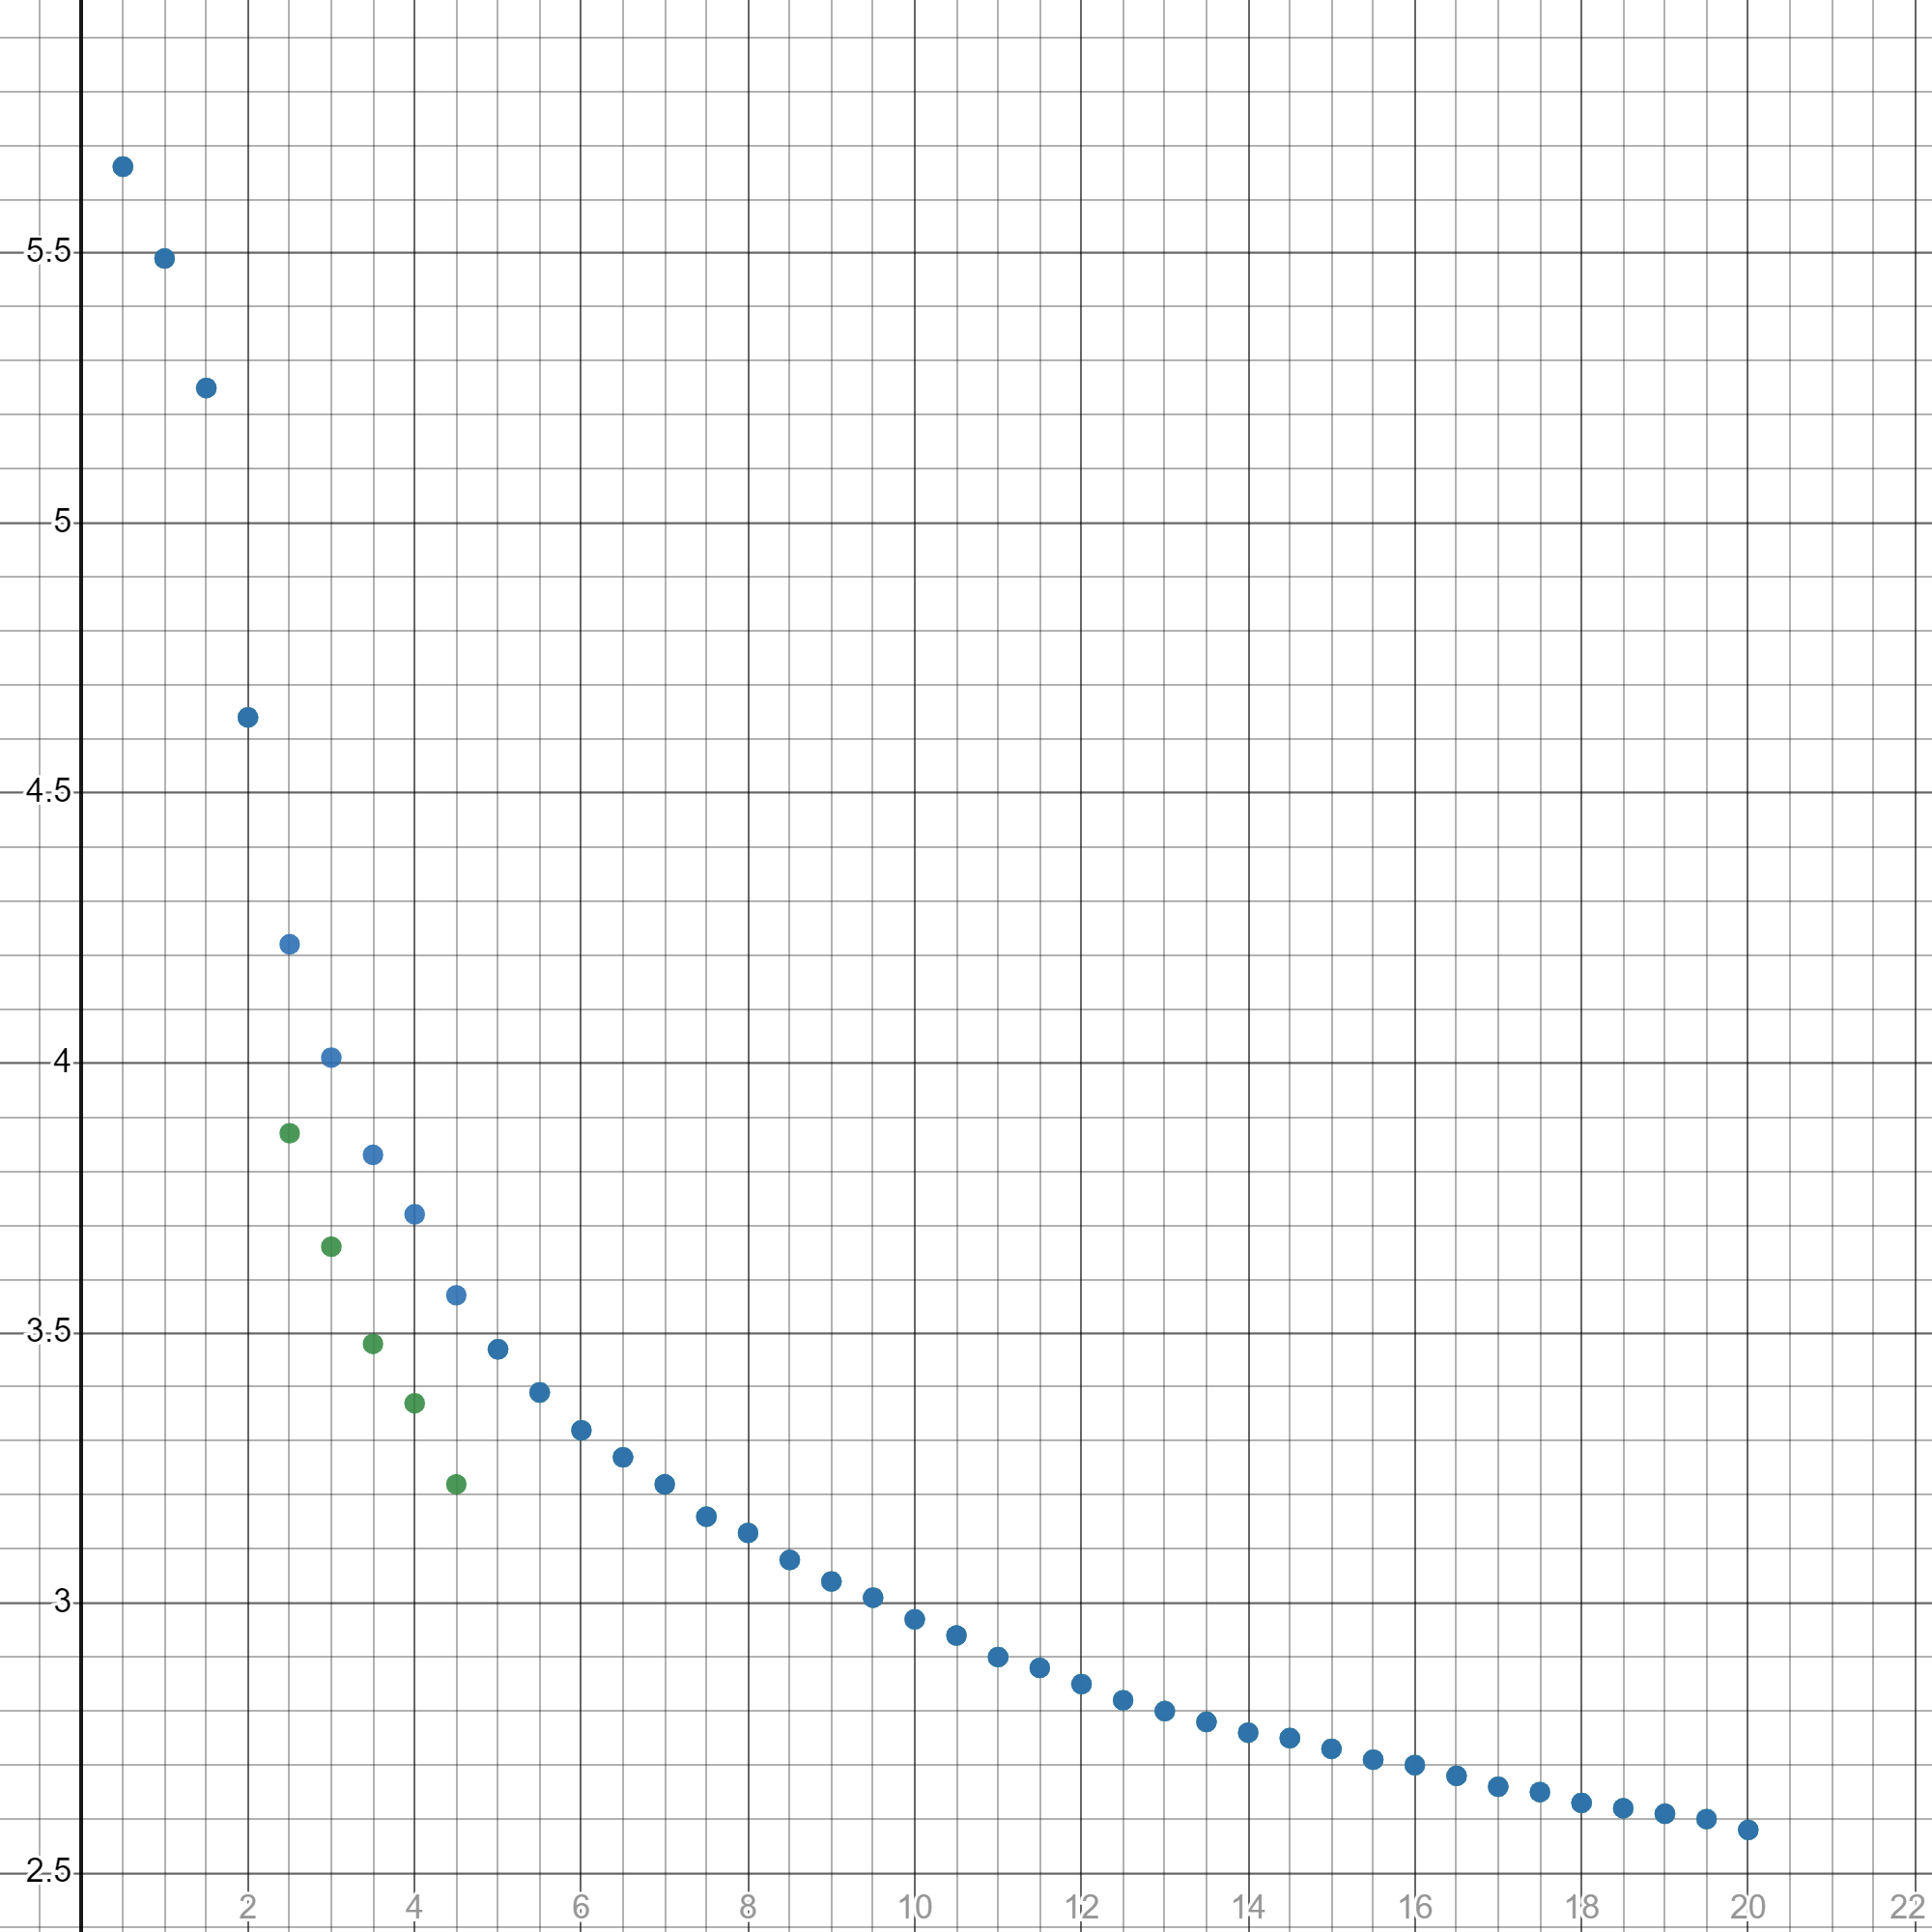
\includegraphics[width=0.7\linewidth]{desmos-graph.png}
     \caption{}
    \label{pn}
\end{figure}

Ксожелениею, растовор получился плохим и поэтому данных с 
$pH\inner{\delta}$ где $\delta$ это объем добавленной соляной кислоты
поэтому растчитать.з уравнения 2.3 можно расчитать определить, что 
коэффицент эквивалентности - 1, буфферную емкость раствора можно 
по формуле:
\begin{equation} 
 p = \cfrac{i\Delta \delta}{\Delta pH} = 0.27 \cfrac{mol}{l\cdot pH}.
\end{equation}    

\end{document}